\chapter{Diseño del sistema}
%
\section{Diseño Conceptual}
%
\subsection{Necesidades - Requerimientos}


Para identificar las áreas funcionales del sistema, se llevó a cabo un análisis de las necesidades y requerimientos. Este análisis se fundamentó en la recopilación de información relevante, obtenida mediante entrevistas y conversaciones con las partes interesadas, así como en el desarrollo iterativo del diseño. El resultado de este proceso es la tabla \ref{tab:NyR}, donde se detallan los requerimientos funcionales y no funcionales que guían el diseño del sistema.

Dicha tabla establece un marco claro para el desarrollo. En ella se especifican las características clave que el sistema debe cumplir para satisfacer tanto las expectativas de los usuarios como los objetivos técnicos del proyecto. A partir de esta base, se definieron criterios que permitirán evaluar el desempeño del sistema en etapas posteriores.

% Please add the following required packages to your document preamble:
% \usepackage{graphicx}
\begin{table}[htbp]
\centering
\caption{Necesidades y requerimientos del sistema}
\label{tab:NyR}
\resizebox{\textwidth}{!}{%
\begin{tabular}{ccc}
\hline
\textbf{Necesidad} &
  \textbf{Requerimiento} &
  \textbf{\begin{tabular}[c]{@{}c@{}}Funcional o \\ No funcional\end{tabular}} \\ \hline
\begin{tabular}[c]{@{}c@{}}Almacenar el alimento de manera que no se vea \\ afectado o deteriorado por el ambiente ni el material\end{tabular} &
  \begin{tabular}[c]{@{}c@{}}El contenedor debe almacenar \\ $23 \text{kg}$ de alimento\end{tabular} &
  F \\ \hline
\begin{tabular}[c]{@{}c@{}}Pesar el alimento en porciones adecuadas de \\ acuerdo a la cantdad de gallinas\end{tabular} &
  \begin{tabular}[c]{@{}c@{}}El alimento debe ser pesado de acuerdo a \cite{Hy-Line}, que \\ indica un promedio de 103g por gallina, al día.\end{tabular} &
  F \\ \hline
\begin{tabular}[c]{@{}c@{}}Transportar y distribuir las porciones \\ de alimento a lo largo de $1.5 \text{m}$\end{tabular} &
  \begin{tabular}[c]{@{}c@{}}El alimento debe ser distribuido de \\ manera uniforme en un espacio \\ máximo de $1.5\text{ m}$; debe \\ realizar la rutina dos veces al día.\end{tabular} &
  F \\ \hline
\begin{tabular}[c]{@{}c@{}}Nidales que no interfieran con el \\ comportamiento natural de las gallinas\end{tabular} &
  \begin{tabular}[c]{@{}c@{}}Los nidales deben adaptarse, tal que, \\ se puedan recoger los huevos desde la \\ parte externa del gallinero, para \\ no afectar su comportamiento\end{tabular} &
  NF \\ \hline
Identificar gallinas &
  \begin{tabular}[c]{@{}c@{}}Se debe poder identificar a las gallinas y \\ su ingreso a los nidales\end{tabular} &
  F \\ \hline
Registro diario de la postura &
  \begin{tabular}[c]{@{}c@{}}Para el registro de postura se debe \\ despreciar materia fecal y paja en los nidales\end{tabular} &
  F \\ \hline
\end{tabular}%
}
\end{table}

\subsection{Arquitectura funcional} \index{arquitectura funcional}


Una vez determinados los requerimientos del sistema, se identifican las funciones que deberá realizar, teniendo entonces:

\textbf{Función principal:}
Alimentar gallinas de postura para que produzcan huevo y monitorizar la postura de cada gallina.

Dicha función se puede tratar como dos funciones principales para simplificar el diagrama de funciones, quedando:

\textbf{Funciones principales:}
\begin{afunc}{FP}
    \item Alimentar gallinas.
    \item Monitorizar postura.
\end{afunc}

De dónde se determinan las siguientes funciones para la función principal, \textbf{Alimentar gallinas}, de la siguiente manera:

\textbf{Funciones secundarias FP 1:}
\begin{afunc}{F}
    \item Comunicar con el usuario.
    \begin{afunc}{F}
        \item Definir cantidad de gallinas.
        \item Ajustar horario de trabajo.
    \end{afunc}
    \item Almacenar alimento.
        \begin{afunc}{F}
            \item Proporcionar alimento.
        \end{afunc}
    \item Medir alimento.
        \begin{afunc}{F}
            \item Pesar alimento mediante sensores.
            \item Transportar alimento para su distribución.
        \end{afunc}
    \item Distribuir alimento.
        \begin{afunc}{F}
            \item Contener alimento.
            \item Mover tolva.
            \begin{afunc}{F}
                \item Dosificar alimento de manera uniforme.
            \end{afunc}
        \end{afunc}
    \item Contener el alimento.
\end{afunc}

Una vez definidas las funciones de \textit{Alimentar gallinas} , se pueden representar en el diagrama de la imagen \ref{fig:AFFP1}. 

\begin{figure}[htbp]
    \centering
    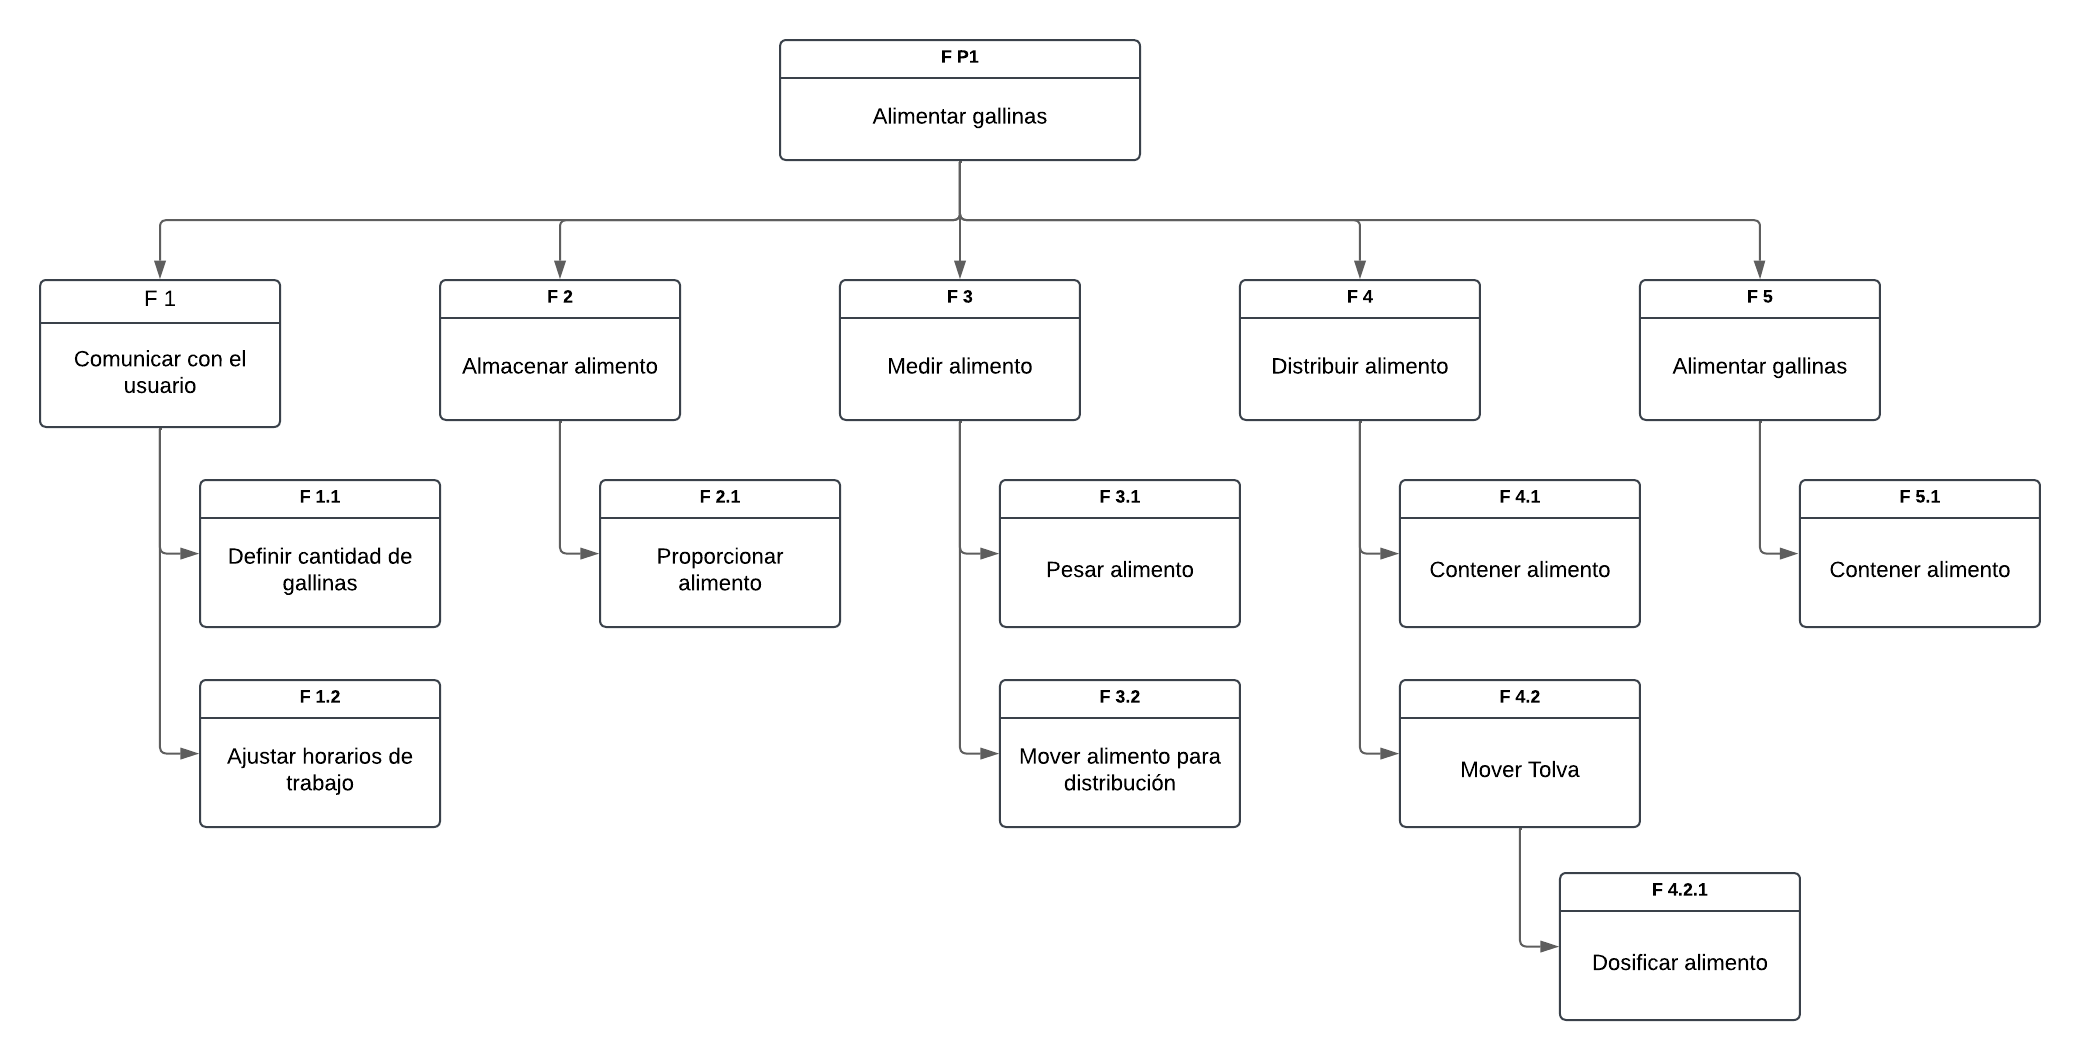
\includegraphics[width=\linewidth]{imagenes/imacap/discon/AFFP1.png}
    \caption{Arquitectura funcional para la función principal de alimentar gallinas.}
    \label{fig:AFFP1}
\end{figure}

Para la función principal, \textbf{Monitorizar postura}, se determinan las siguientes funciones:

\textbf{Funciones secundarias FP 2:}
\begin{afunc}{F}
    \item Comunicar con el usuario.
    \begin{afunc}{F}
        \item Identificar gallinas improductivas.
        \item Mostrar registro de postura.
    \end{afunc}
    \item Registrar postura.
    \begin{afunc}{F}
        \item Identificar gallina.
        \item Identificar postura.
        \item Registrar postura de huevo.
        \item Comunicar con el maestro.
    \end{afunc}
\end{afunc}

\begin{figure}[htbp]
    \centering
    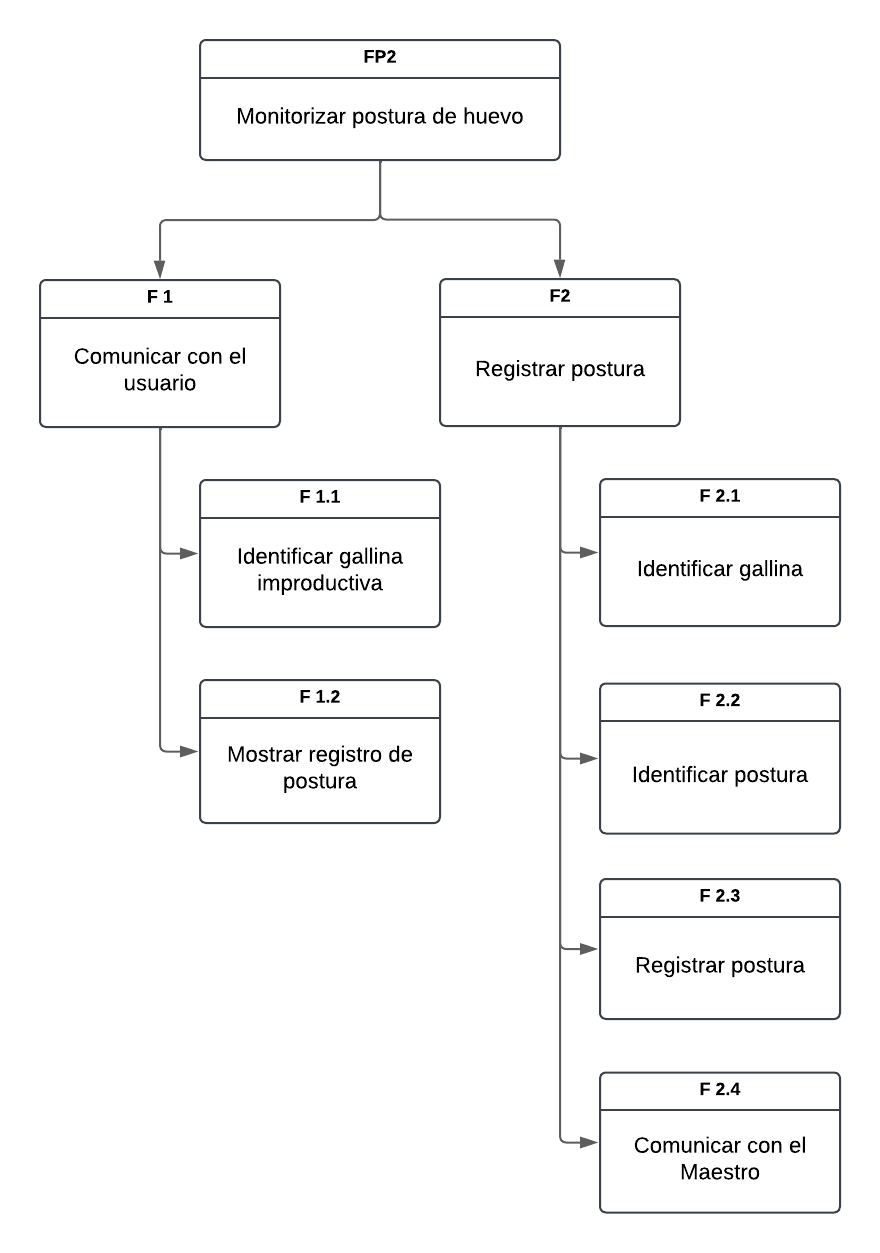
\includegraphics[width=0.5\linewidth]{imagenes/imacap/discon/AFFP2.png}
    \caption{Arquitectura funcional para la función principal de registrar la postura de huevo.}
    \label{fig:AFFP2}
\end{figure}

%A partir de éste punto y en adelante se tratará al sistema como dos subsistemas independientes, relacionados entre sí. A fin de evitar confusión, se les llamará sistemas.
\newpage
\subsection{Arquitectura física}

Una vez definidas las funciones, se establecen los módulos que compondrán el sistema, identificando así la estructura y relación que tendrán entre ellos.

Para el sistema de alimentación se tienen los módulos:

\begin{afunc}{M}
    \item Comunicación Humano-Máquina.
    \item Estructura de almacenamiento.
    \item Módulo de pesaje del alimento.
    \item Distribución y alimentación.
    \item Control del sistema de alimentación.
\end{afunc}

Mientras que para el sistema de registro de postura se tienen los módulos:

\begin{afunc}{M}
    \item Comunicación Humano-Máquina.
    \item Detección y registro de postura.
\end{afunc}

Obteniendo entonces la imagen \ref{fig:AFS}, en la que se muestran las relaciones entre cada uno de los módulos, identificando las entradas y salidas de cada uno. 

\begin{figure}[htbp]
    \centering
    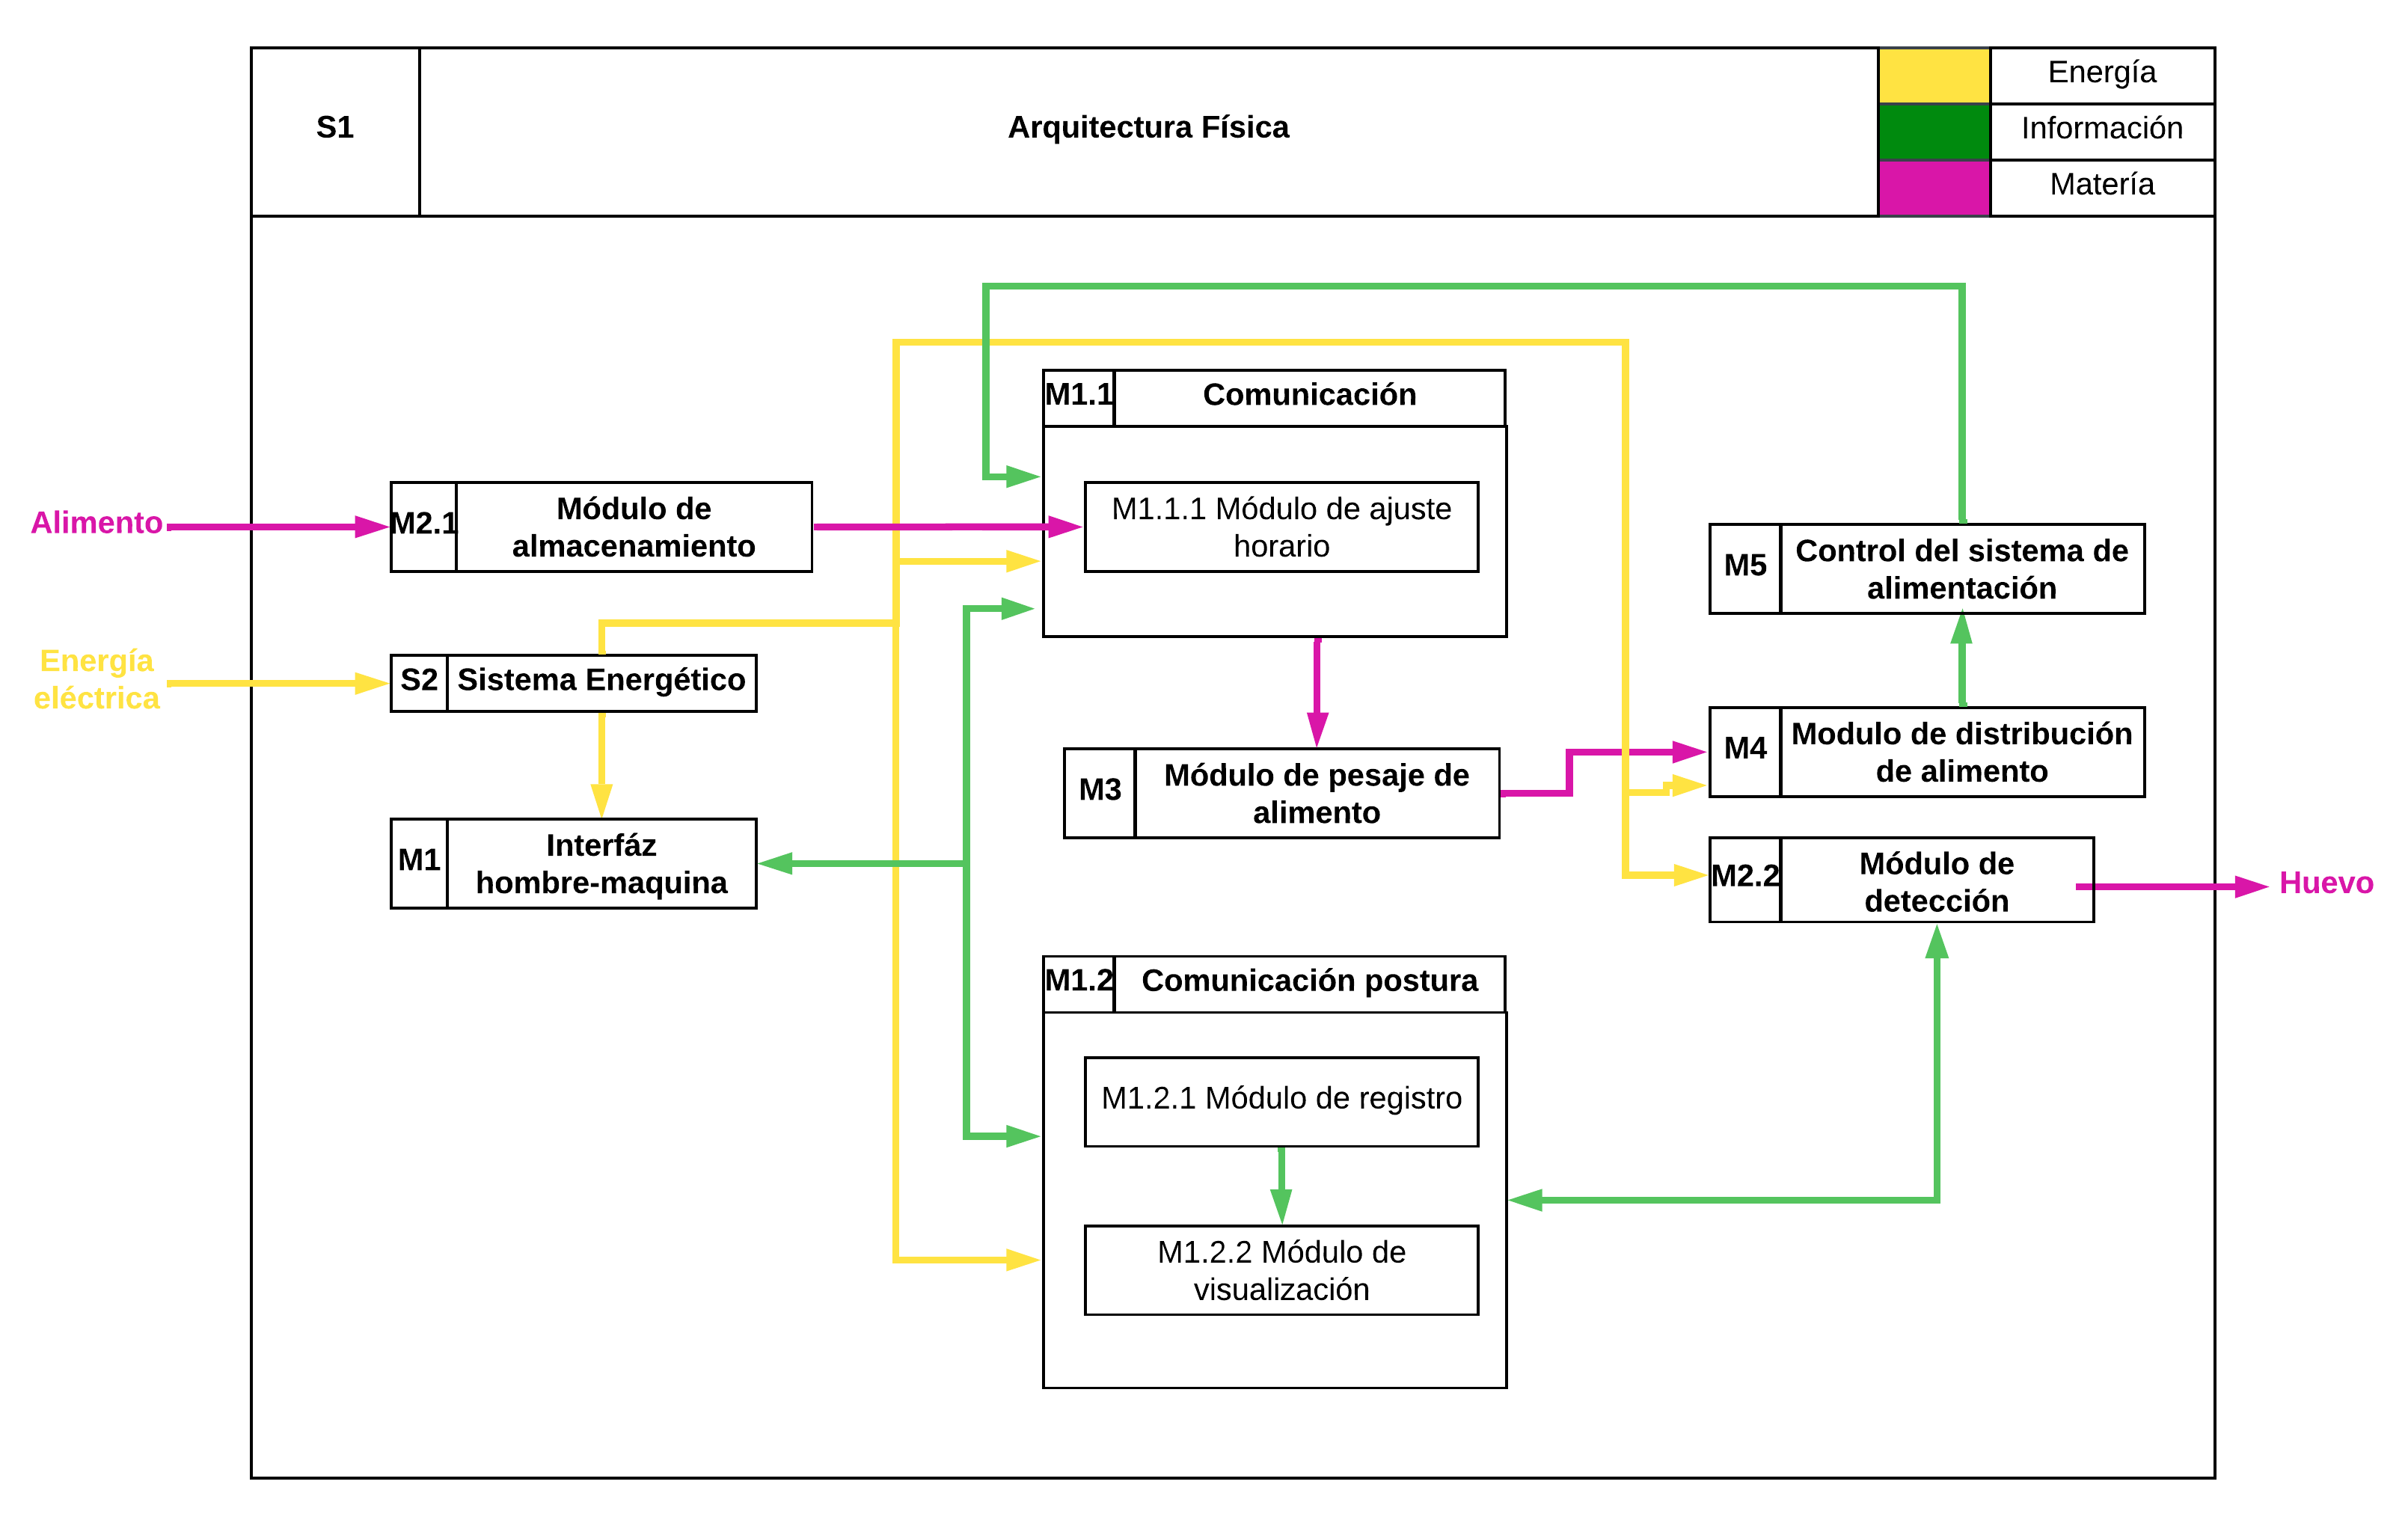
\includegraphics[width=\linewidth]{imagenes/imacap/discon/Arquitectura fisica.png}
    \caption{Arquitectura física del sistema de alimentación.}
    \label{fig:AFS}
\end{figure}

\newpage

\subsection{IDEF-0}

Una vez establecidas las necesidades, los requerimientos, las funciones y los módulos del sistema, se elaboró el modelo IDEF-0 para establecer la arquitectura física del sistema, que apoyará en la identificación de los sistemas de control y los mecanismos que serán necesarios. Los diagramas de las imágenes \ref{fig:IDEF0A-0}, \ref{fig:IDEF0A0},\ref{fig:IDEF0A01} y \ref{fig:IDEF0A2}, muestran los nodos del modelo IDEF-0.

\begin{figure}[htbp]
    \centering
    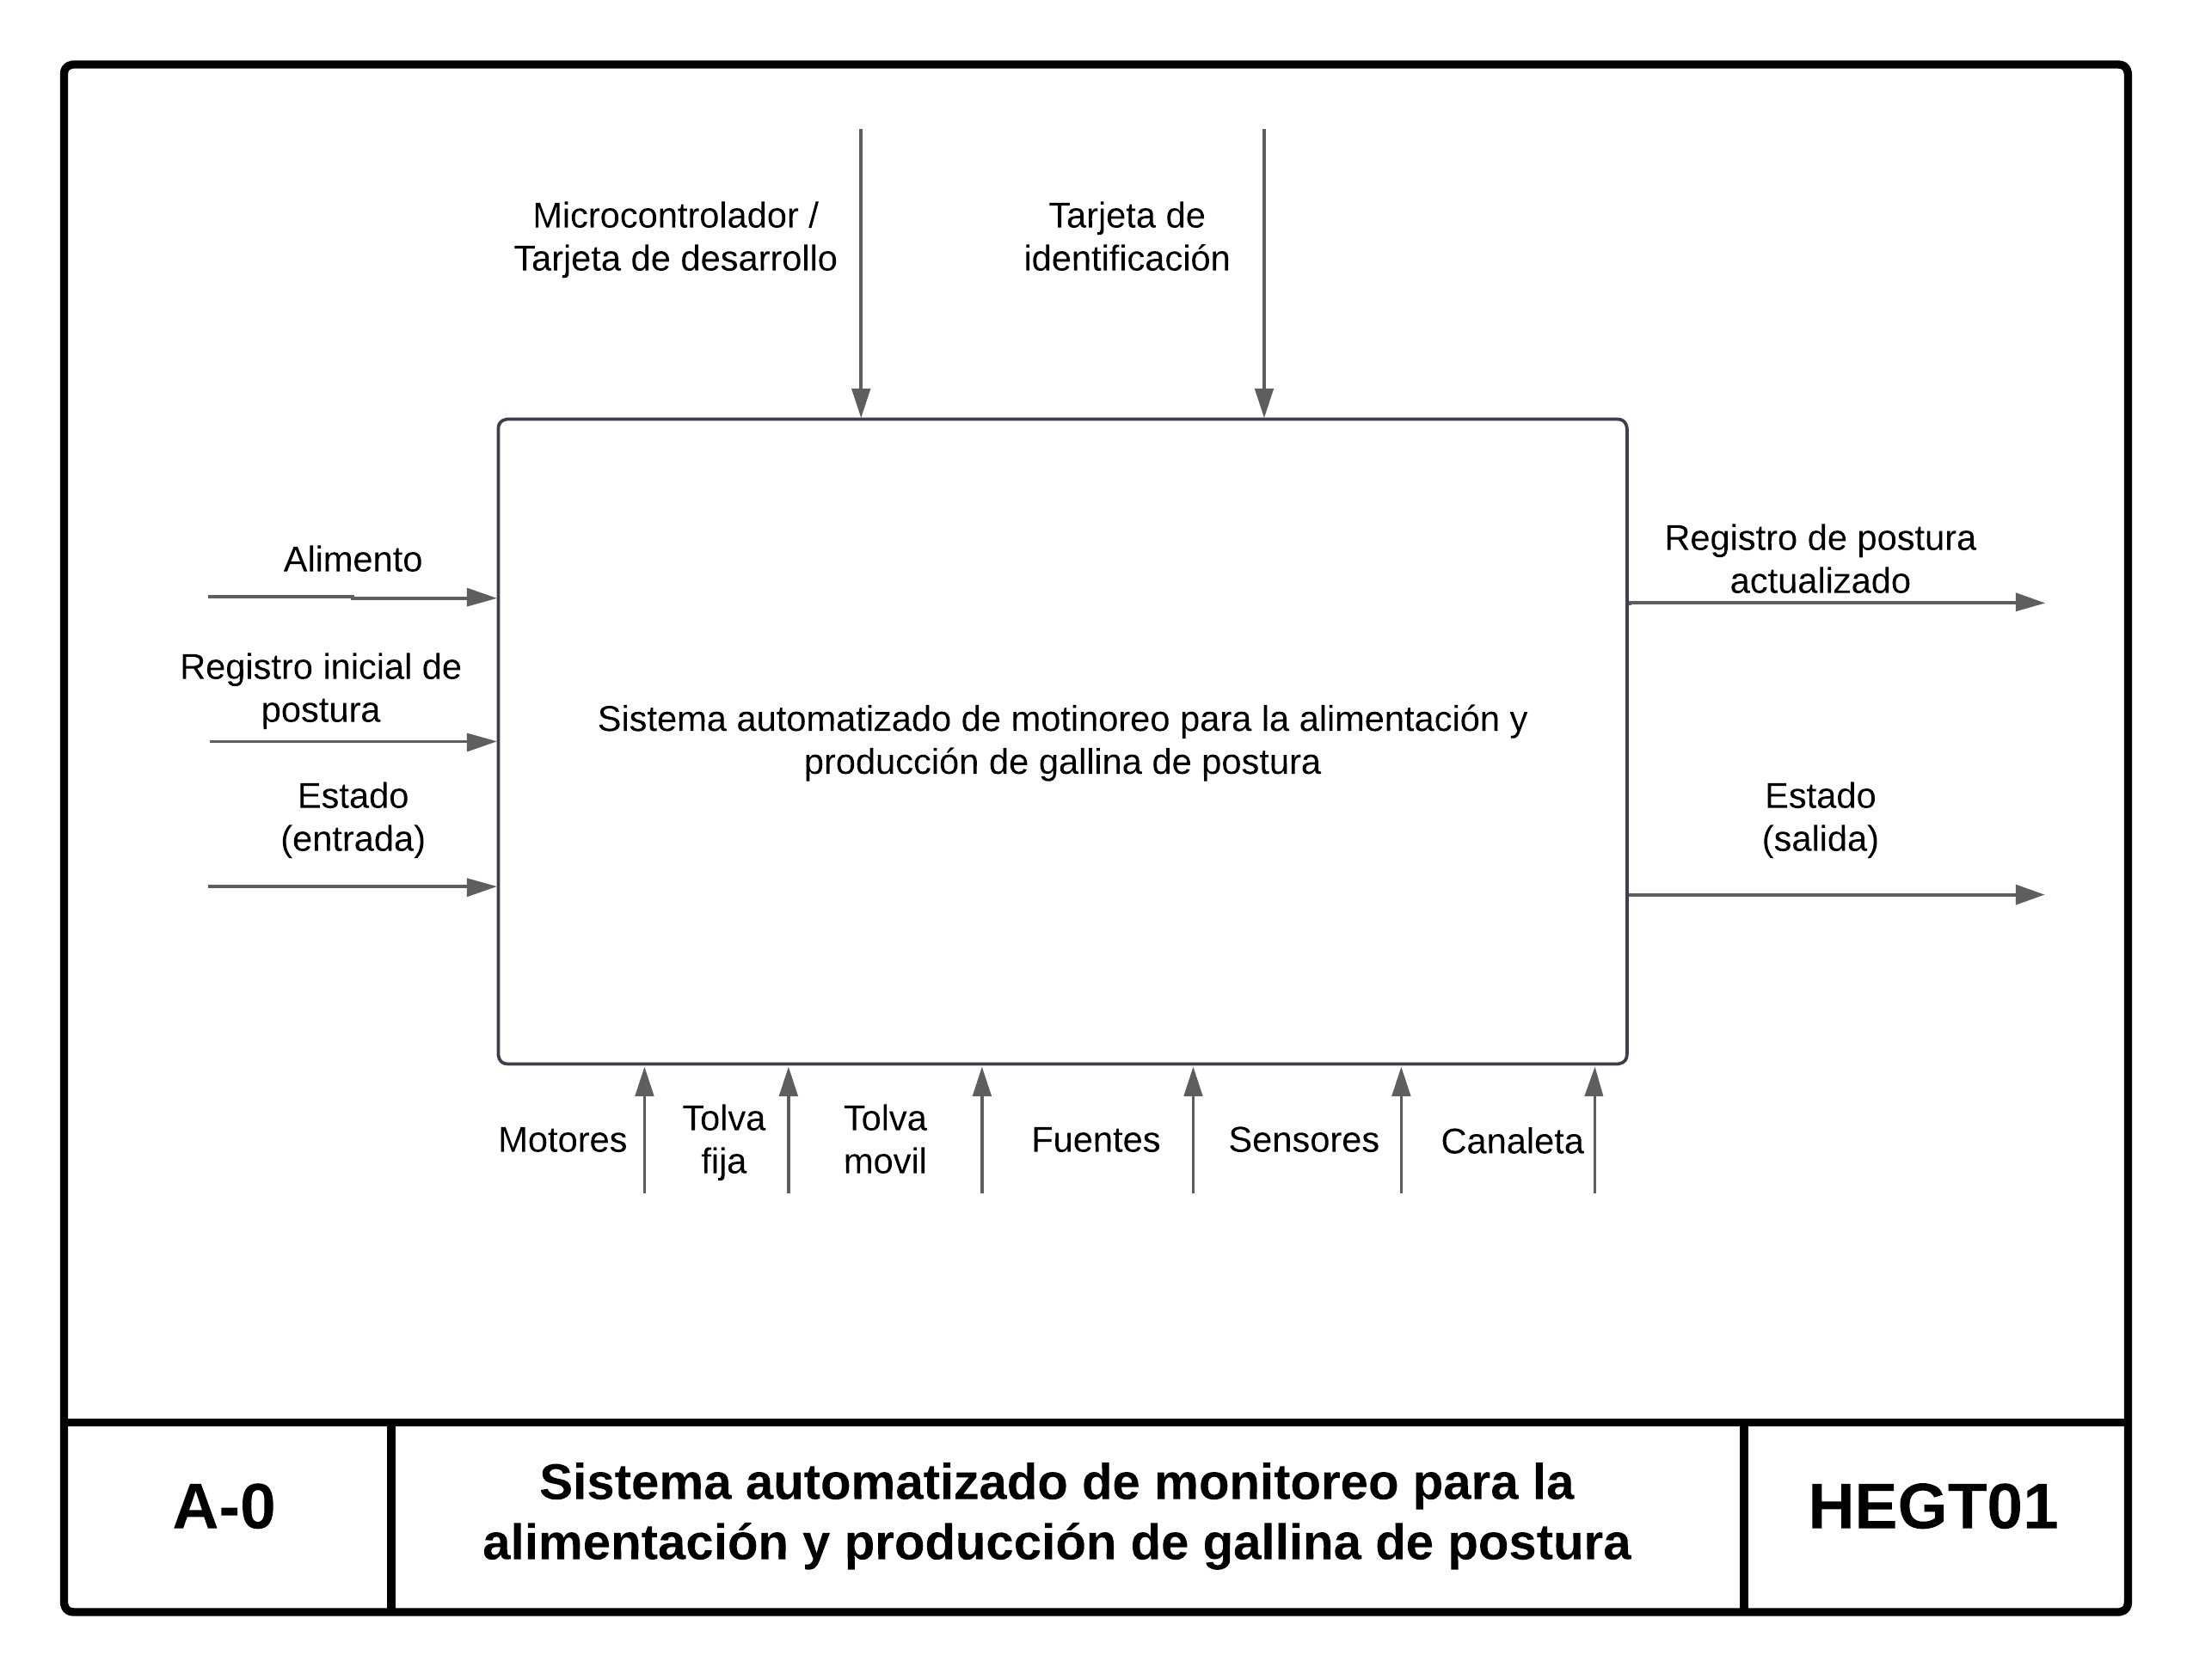
\includegraphics[width=\linewidth]{imagenes/imacap/discon/A-0.png}
    \caption{IDEF-0, Nodo A-0}
    \label{fig:IDEF0A-0}
\end{figure}

\begin{figure}[htbp]
    \centering
    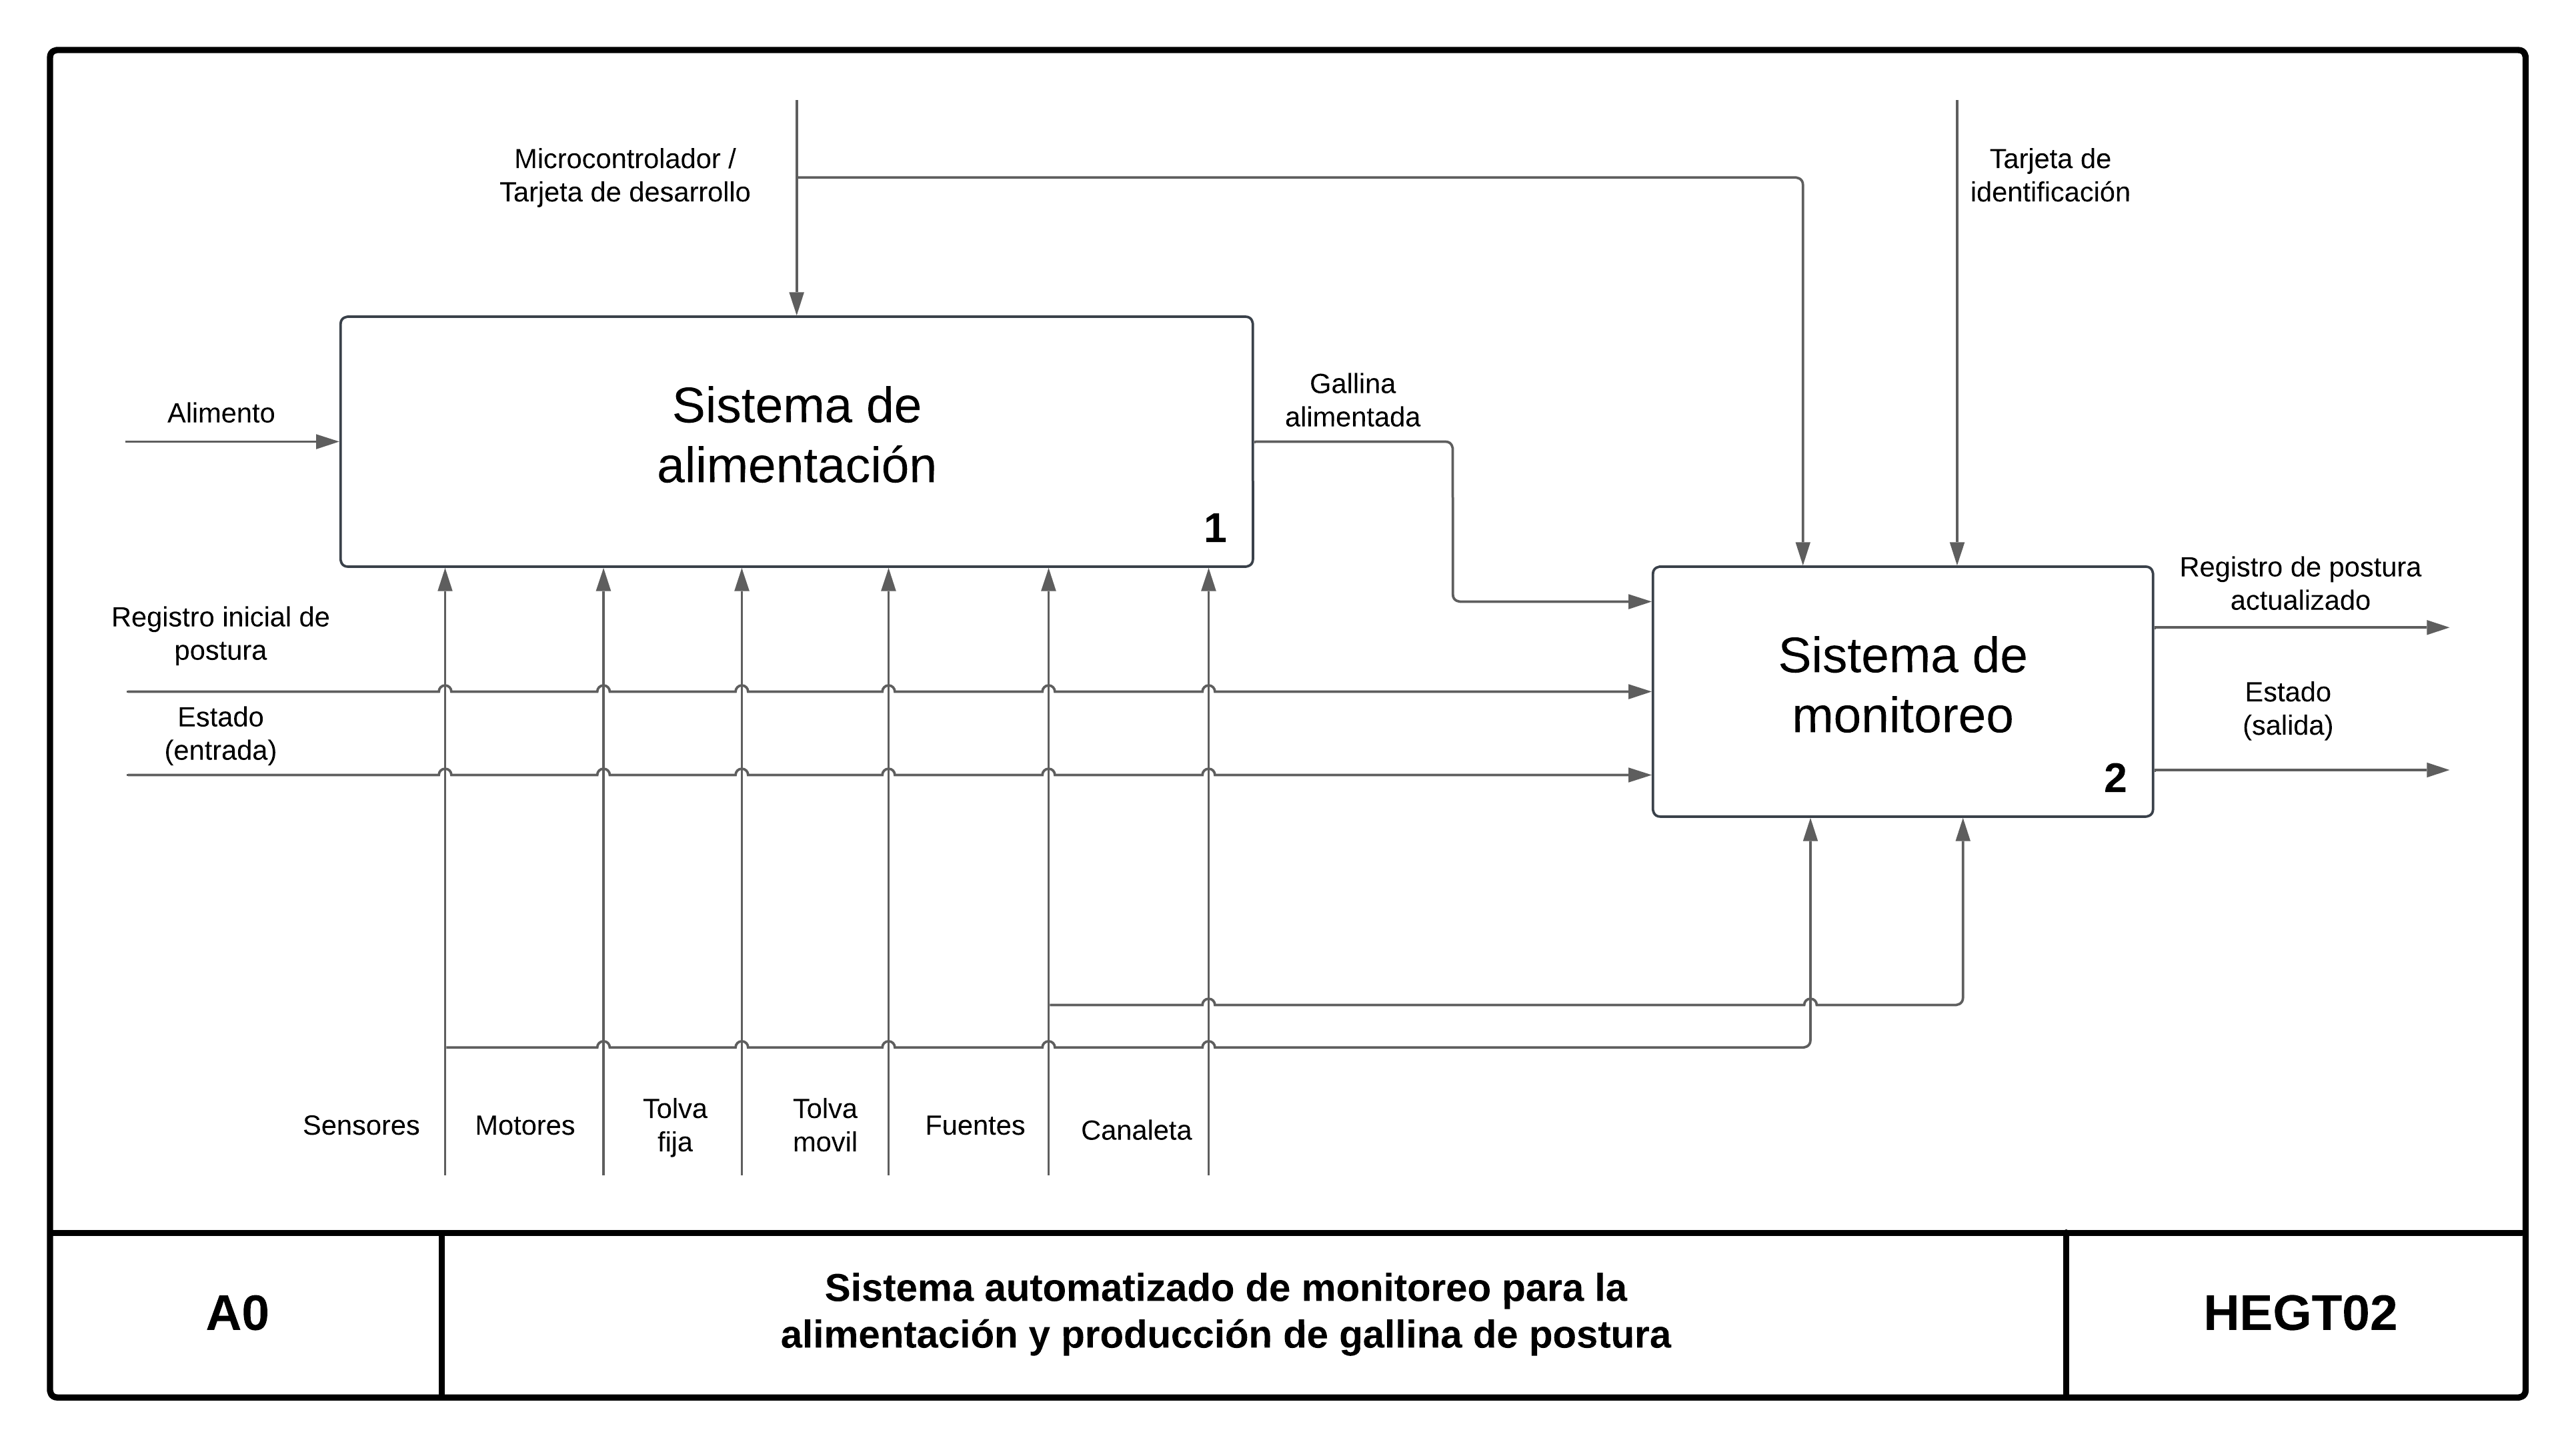
\includegraphics[width=\linewidth]{imagenes/imacap/discon/A0.png}
    \caption{IDEF-0, Nodo A0}
    \label{fig:IDEF0A0}
\end{figure}

\begin{figure}[htbp]
    \centering
    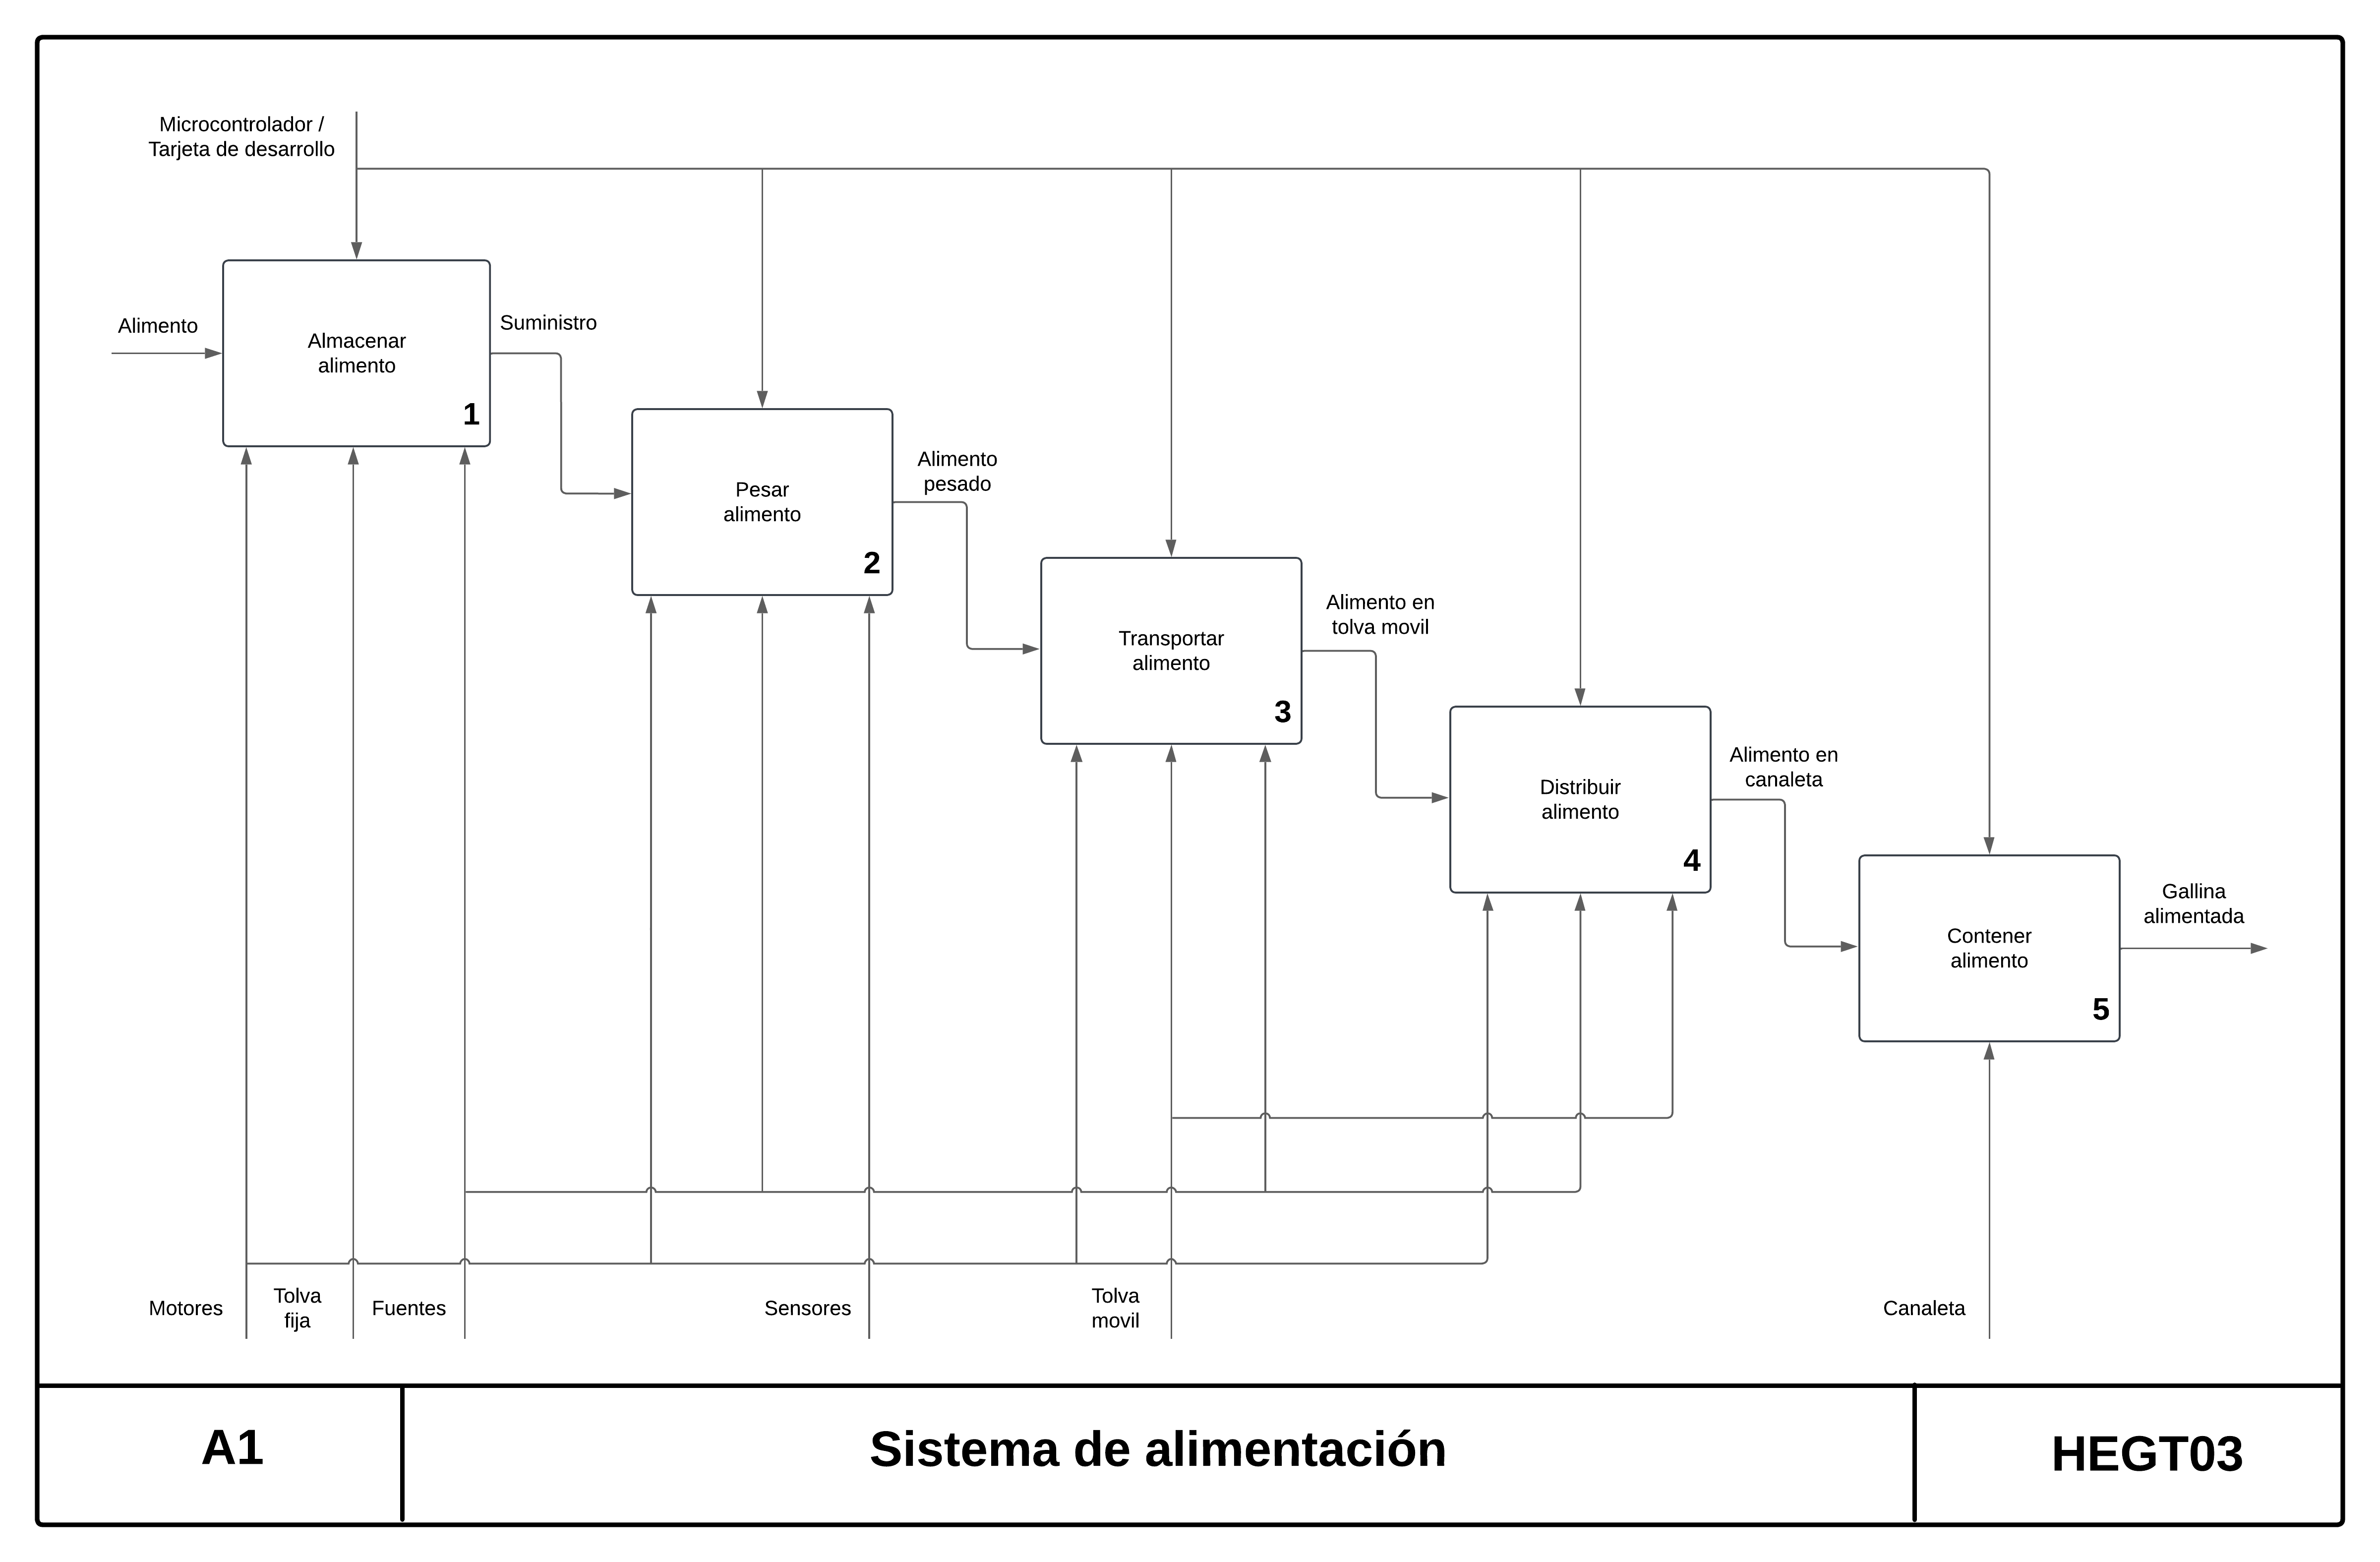
\includegraphics[width=\linewidth]{imagenes/imacap/discon/A1.png}
    \caption{IDEF-0, Nodo A1}
    \label{fig:IDEF0A01}
\end{figure}


\begin{figure}[htbp]
    \centering
    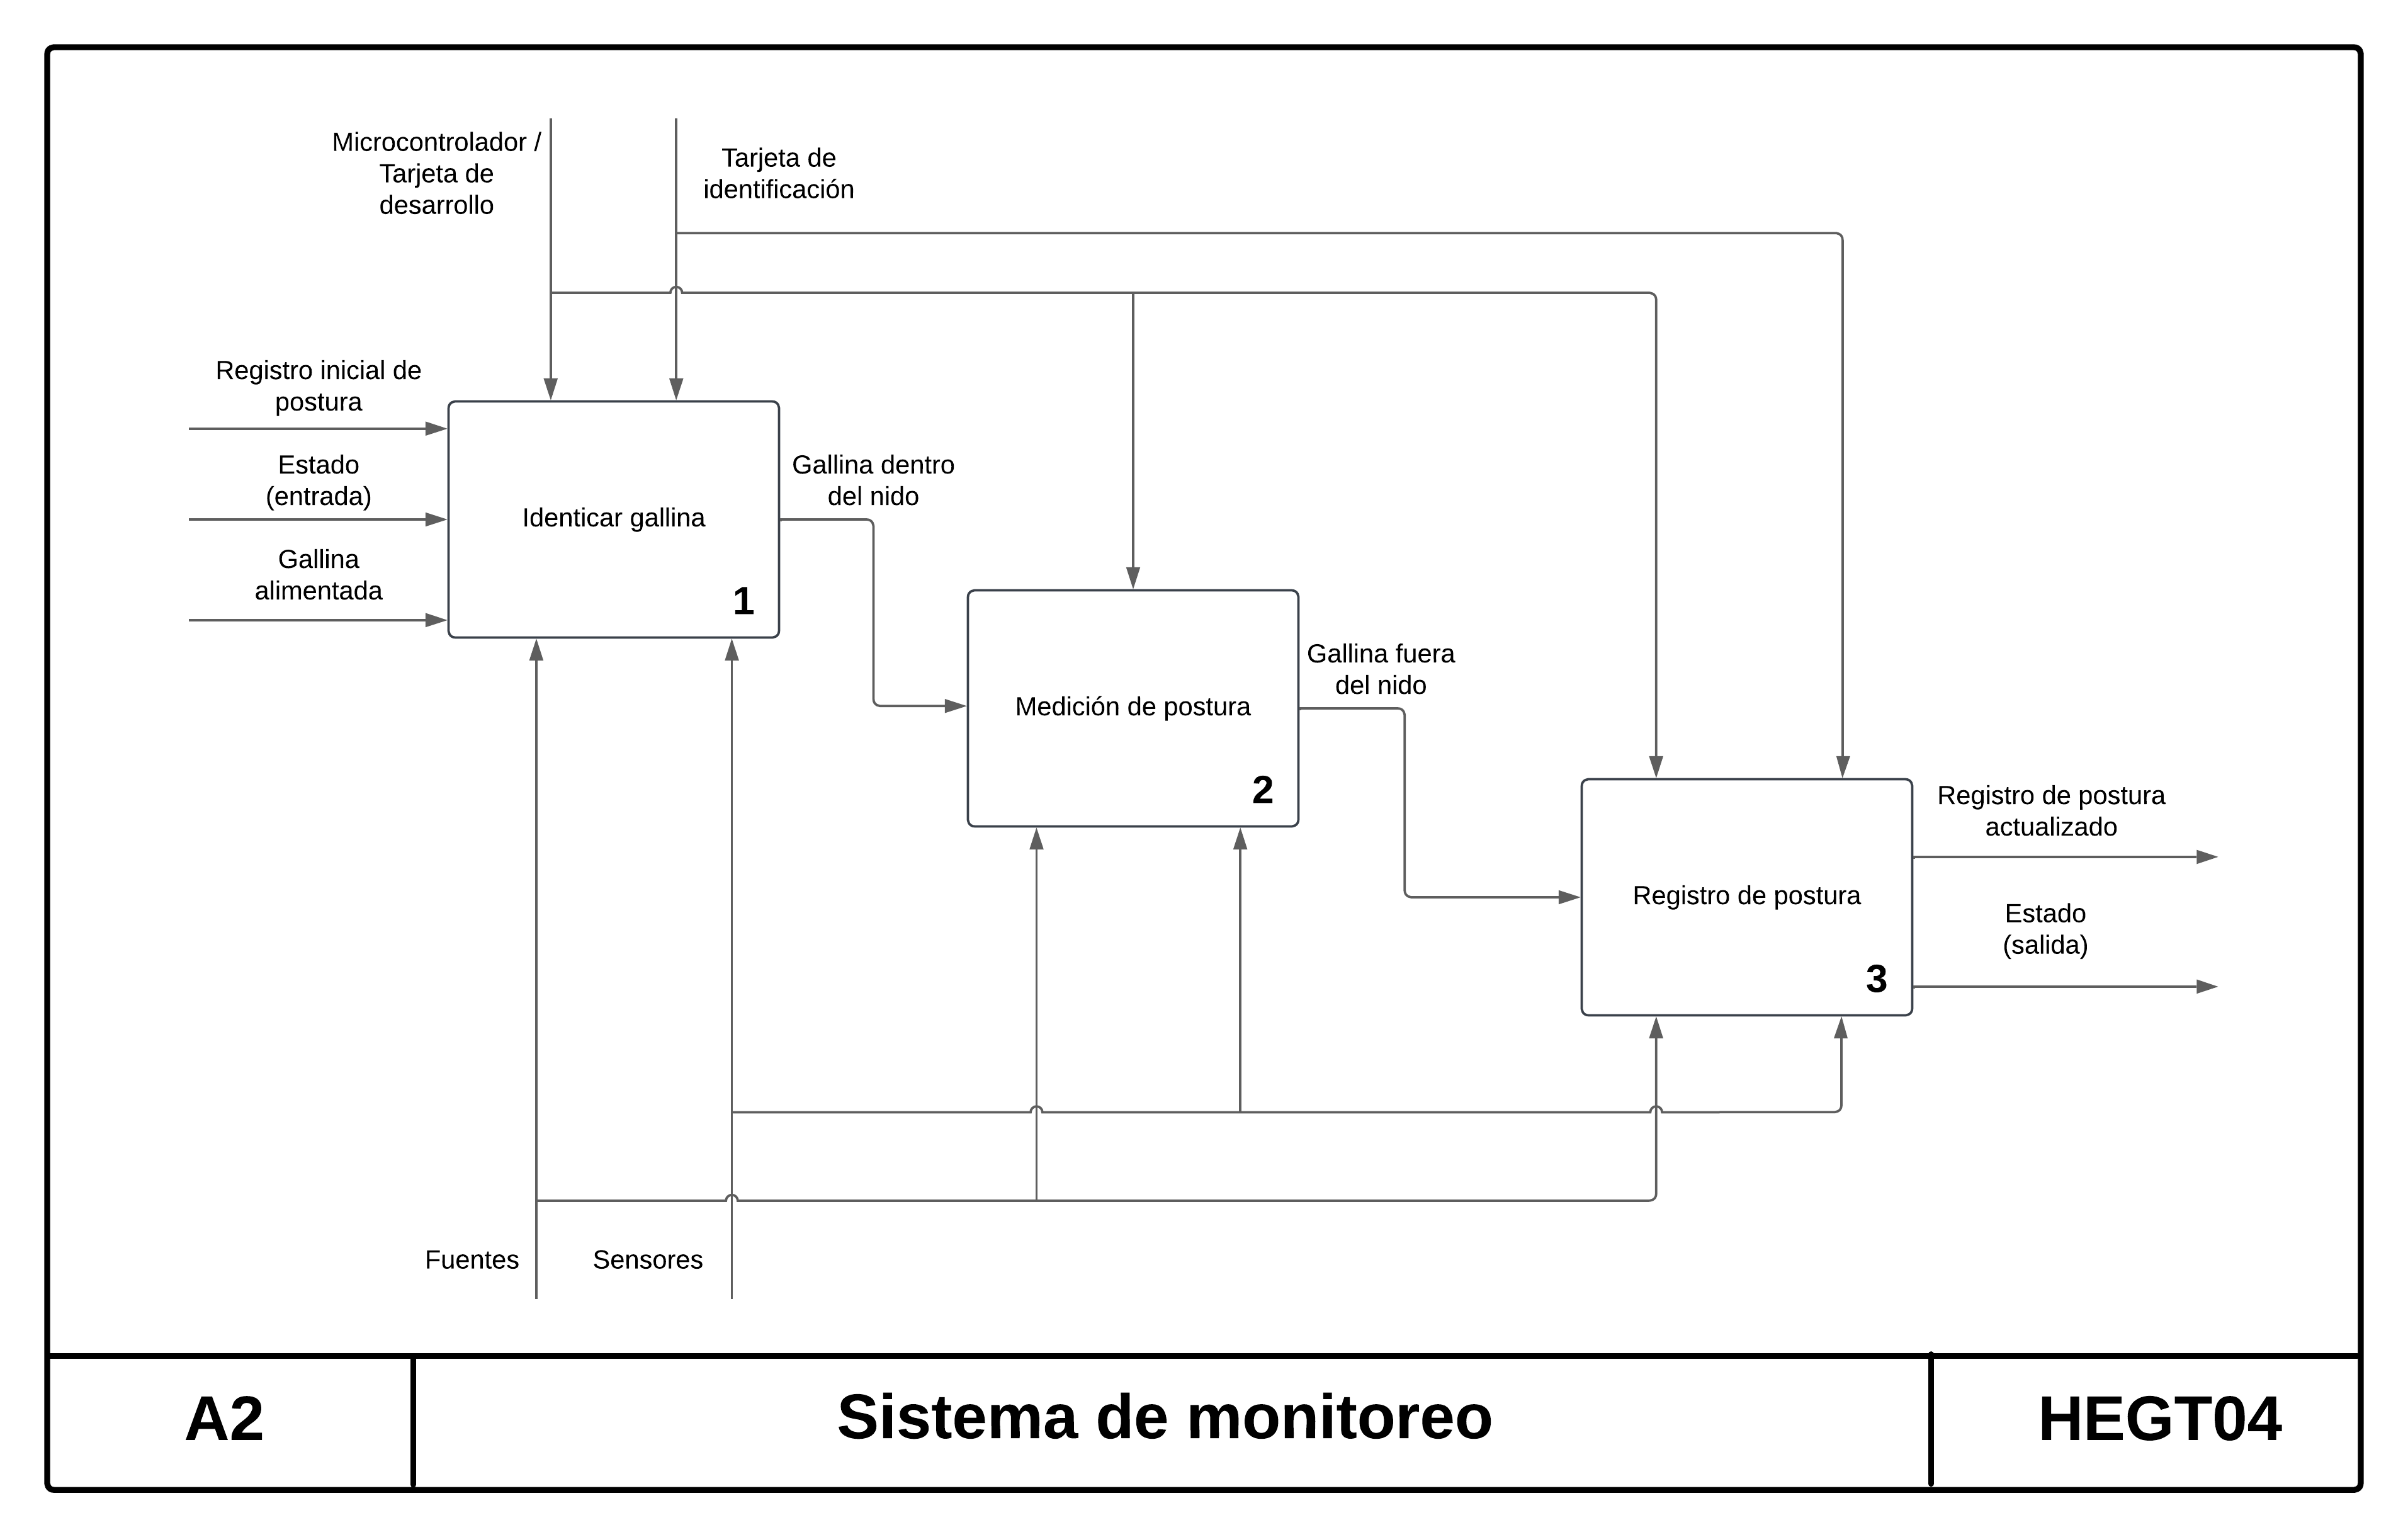
\includegraphics[width=\linewidth]{imagenes/imacap/discon/A2.png}
    \caption{IDEF 0, Nodo A2}
    \label{fig:IDEF0A2}
\end{figure}
%En el subsistema de alimentación se identificó como entrada de la función principal, el alimento; como control, microcontrolador/tarjeta de desarrollo; para los mecanismos o  se encontraron necesarios báscula, motores, tolva fija, tolva móvil y fuente de CD; en la salida tener a las gallinas alimentadas. Obteniendo así el diagrama de la imagen \ref{fig:IDEF0Alim}.

\newpage

\subsection{Propuestas de solución}

Para la solución del problema, primero, se propone el diseño de un alimentador automático que funcione de acuerdo al diagrama de flujo de la imagen \ref{fig:DFSA}. 

\begin{figure}[htbp]
    \centering
    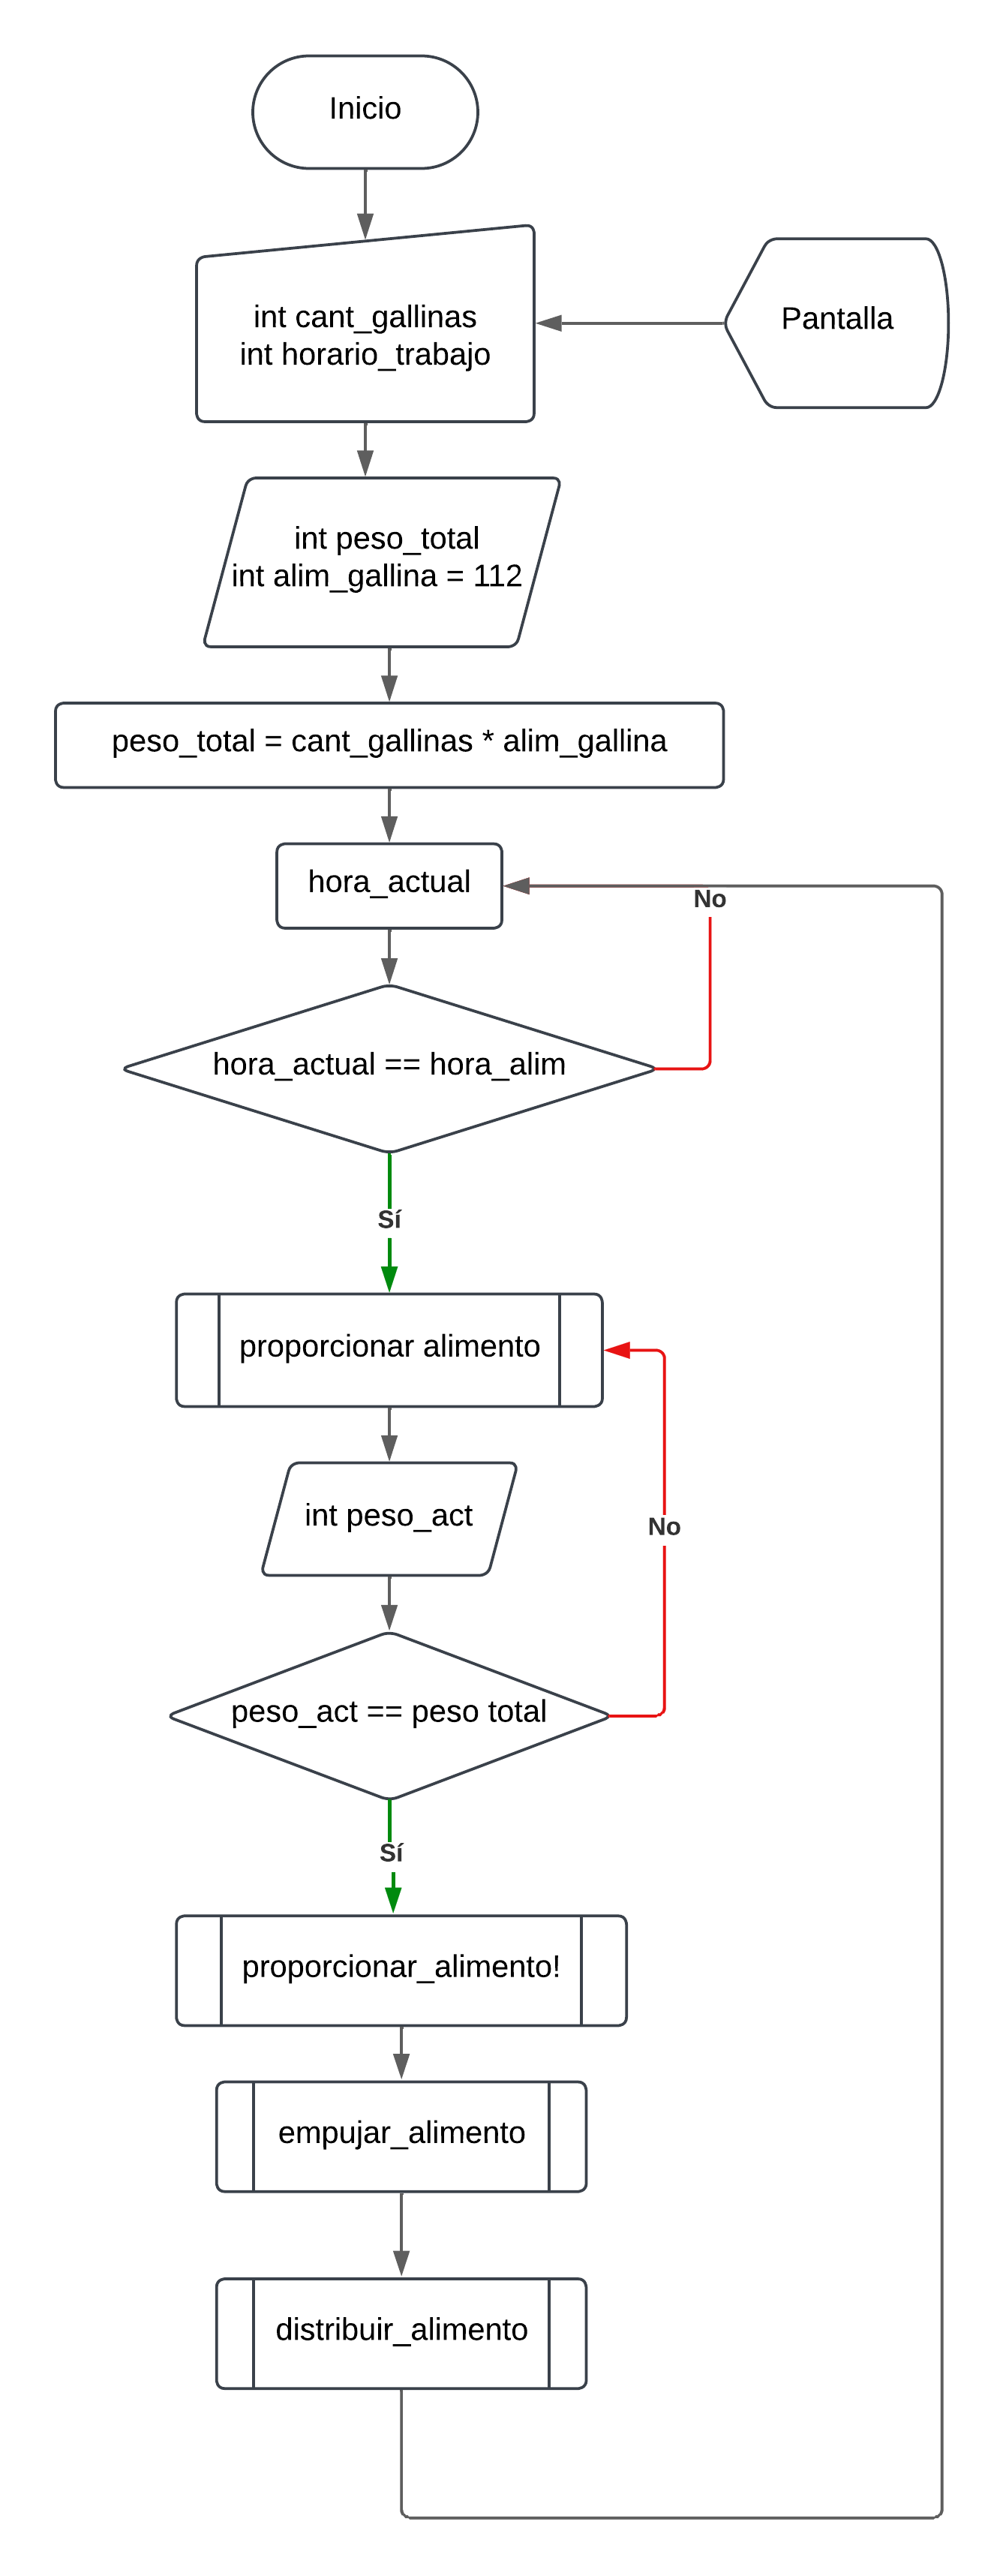
\includegraphics[width=0.36\linewidth]{imagenes/imacap/discon/DFSA.png}
    \caption{Diagrama de flujo funcionamiento general del sistema de alimentación.}
    \label{fig:DFSA}
\end{figure}

\newpage
En el caso del sistema de monitoreo de postura, se propone el diagrama de flujo de la imagen \ref{fig:DFSM}.

\begin{figure}[htbp]
    \centering
    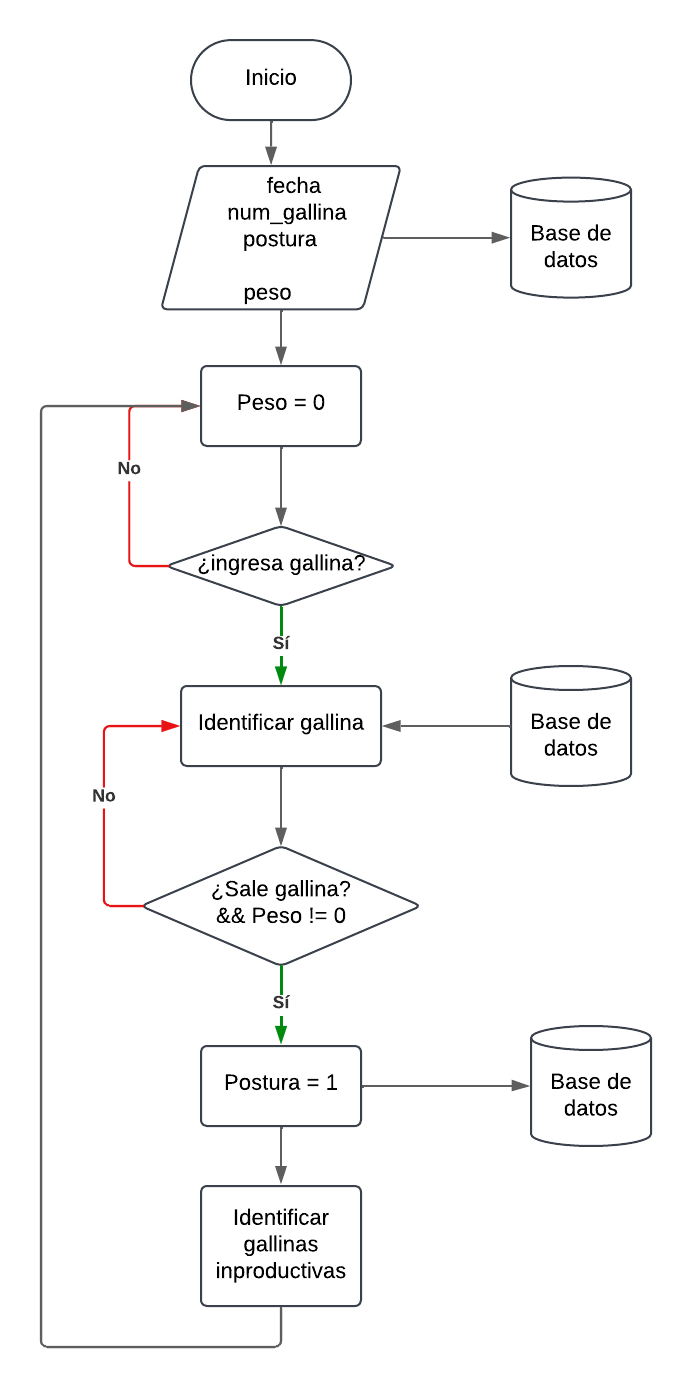
\includegraphics[width=0.46\linewidth]{imagenes/imacap/discon/DFR.png}
    \caption{Diagrama de flujo funcionamiento general del sistema de monitoreo.}
    \label{fig:DFSM}
\end{figure}

%\subsubsection{Integración (sistema)}

%\subsection{Validación}

%\subsection{Selección diseño conceptual}



%%%%%%fin del archivo
\endinput